\section{Results and Discussion}\label{sec:Discussion}
\subsection{Sampling of States using Metropolis}

\begin{figure}
	\begin{subfigure}{\textwidth}
		\centering
		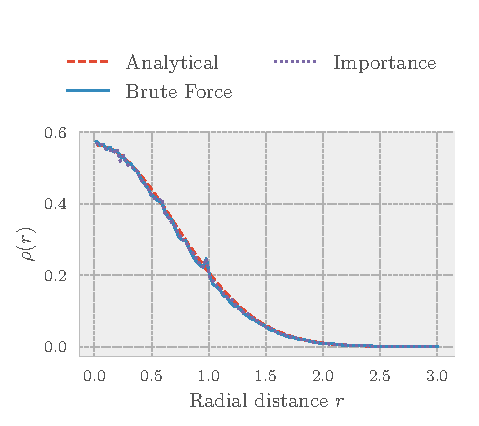
\includegraphics[width=.8\linewidth]{figures/density1.pdf}
		\subcaption{Approximation of onebody density using Metropolis brute force sampling vs analytical(kilde)}
		\label{fig:sfig1}
	\end{subfigure}%
	\begin{subfigure}{\textwidth}
		\centering
		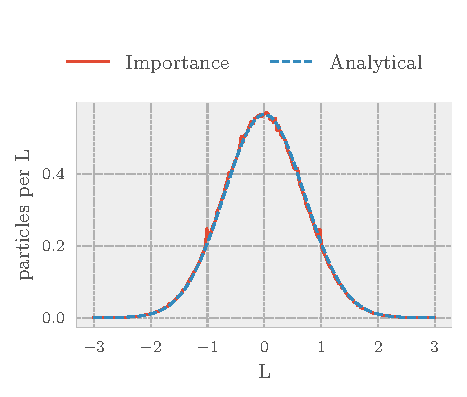
\includegraphics[width=.8\linewidth]{figures/density2.pdf}
		\subcaption{Approximation of onebody density using Metropolis importance sampling vs analytical}
		\label{fig:sfig2}
	\end{subfigure}
	\caption{One-body density of 1 boson in 1 dimmension, using $N = 1e6$ cycles, $\omega = 1$, $\alpha = 0.5$.}
	\label{fig:1 part 1 dim density}
\end{figure}

\begin{figure}
	\begin{subfigure}{\textwidth}
		\centering
		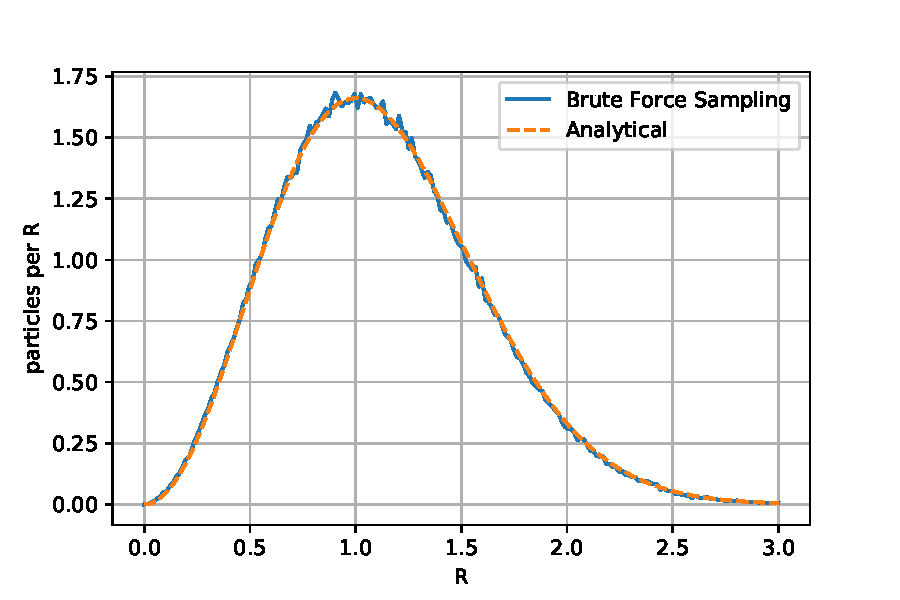
\includegraphics[width=.8\linewidth]{figures/density3.pdf}
		\subcaption{Approximation of radial onebody density using Metropolis brute force sampling vs analytical}
		\label{fig:sfig1}
	\end{subfigure}%
	\begin{subfigure}{\textwidth}
		\centering
		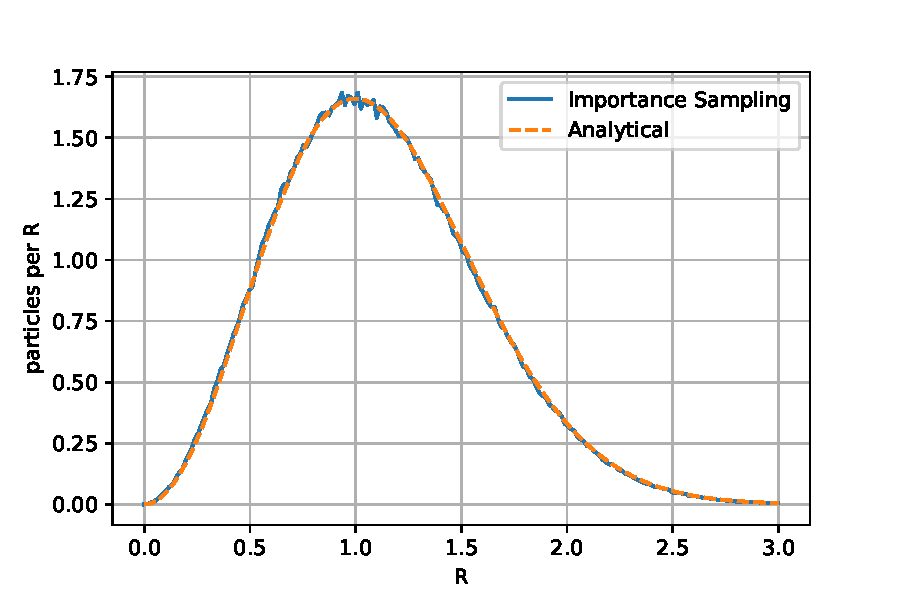
\includegraphics[width=.8\linewidth]{figures/density4.pdf}
		\subcaption{Approximation of radial onebody density using Metropolis importance sampling vs analytical}
		\label{fig:sfig2}
	\end{subfigure}
	\caption{Radial one-body density of 2 non-interacting bosons in 3 dimmensions, using $N = 1e6$ cycles, $\omega = 1$, $\alpha = 0.5$.}
	\label{fig:2 part 3 dim density}
\end{figure}

In \autoref{fig:1 part 1 dim density}  we see that both brute force sampling and importance sampling manage to approximate the onebody density derived from the non-interacting trial wave function: Aside from the statistical noise introduced by the finite number of Monte-Carlo cycles, the approximated densities follow the analytical result closely. Figure \autoref{fig:2 part 3 dim density} demonstrates that this also scales to more particles and dimensions, as seen from the radial onebody density of two particles in three dimensions. 


\subsection{Local Energy and Blocking}

\subsection{Interacting Potentials}
\subsection{Local Energy}
\subsection{Optimal Parameter \(\alpha\)}
\subsection{Onebody Density}

